\chapter{TLMSimulator Co-Simulation \\Framework}
\label{framework}
A general framework for composite modeling and co-simulations has previously been designed~\cite{Siemers+Nakhimovski+Fritzson-05}. 
The design goals for the simulation part of the framework were portability, simplicity to incorporate new simulation tools, and computational efficiency.
These goals were realized by defining the following concepts and interfaces:

\textbf{External interface.} 
A named point on a mechanical object where position and velocity can be evaluated and reaction load (force and moment) applied. 
To guarantee numerical stability when utilising different numerical solvers in the co-simulation, only interfaces based on the {\em transmission line modelling} method, see Section~\ref{secTLMtheory}, are currently supported.

%\item
\textbf{Simulation manager.} 
The central simulation engine. 
It is a stand alone program that reads an XML definition of the coupled simulation.  
It then starts \emph{external model simulations} and provides the communication bridge between the running simulations. 
The external models only communicate with the simulation manager which acts as a broker marshalling information between the external models. 
Simulation manager sees every external model as a black box having one or several external interfaces. 
The information is then forwarded between external interfaces belonging to different external models. 
Additionally the simulation manager opens a network port for monitoring all communicated data.

%\item
\textbf{Interface plug-in.} 
A small C++ library having a single abstract class representing external interface for a specific simulation tool. 
The interface plug-in can be seen by an external model simulator as an external load that depends on position, velocity
and time. 
The implementation of the plug-in handles the necessary communications with the simulation manager. 
It also handles necessary coordinate system transformations into the global composite model inertial system. 
All positions and velocities are transformed from the external-model (simulation-tool specific) inertial system to the
global composite model inertial system. 
All reaction loads are translated back into the local inertial system. 
This constant transformation is stored in the composite model and sent to the corresponding interface plug-in on simulation start up.
%\item

\textbf{External model simulator.} 
Any simulation program that has incorporated the interface plug-in as a part of its model. 
A small script that takes the general parameters as input and starts the specific simulation tool is an additional requirement. 
This intermediate step is necessary since the simulation manager needs a common way to start all the components and each tool might have some specific start procedures.
%\end{itemize}

\section{Graphical User Interface}
The TLMSimulator in itself provides no graphical user interface.
Simulations are started by command line calls to the simulation manager.
However, graphical user interface exists both in SKF BEAST and OpenModelica Connection Editor (OMEdit) \cite{alachew2015}. 


\section{Requirements on External Model Simulators}
\label{sec:requirements}
External models are associated with specialised simulation tools. 
Even though many simulation tools have interfaces to external functions, the interfaces differ between tools. 
Therefore it is first necessary that a software developer who is familiar with the particular tool architecture, designs and implements the {\em external interface} for each tool. 
That is, to create a tool specific wrapper for the {\em interface plug-in} of the simulation framework.

The following functionality is required from all simulation tools that implement the interface plug-in and want to participate in
co-simulation:
\begin{itemize}
\item 
Possibility to start simulation externally or in batch mode.
The developer of the tool specific interface must provide a start up program. 
This is used by the simulation manager to set-up global simulation parameters, that is, start time, end time, and max time step for each co-simulation participant. 
Regarding the maximum time step length: The current co-simulation communication protocol is based on the {\em transmission line modelling} method, see Section~\ref{secTLMtheory} for details. 
This method requires a certain communication time control, i.e., time steps need to be within a physically motivated limit.

\item 
Possibility to integrate the {\em interface plug-in} into the tool specific adaptor. 
Note that the tool independent part of the plug-in is implemented in C++. 
Some tools require external functions to be implemented in, e.g., C or Fortran. 
In such cases the C++ code can be invoked from a C or Fortran function.

\item 
Ability to deliver position, orientation and velocity of a point to the {\em interface plug-in} and receive the reaction load (force and moment) to be applied at this point.

\item 
Ability to send information about the taken solver steps to the interface. 
This is important for variable time step solvers. 
Data is send from one co-simulation party to the other when a time step is completed, that is, if the solver, after many iterations, decided what step it will take next. 
This information needs to be send to the TLMPlugin.

\item 
Correct handling of shutdown signals coming from the tool specific wrapper. 
In some cases the {\em simulation manager} needs to	take down the simulation tool in a controlled way. 
This can be	achieved by a tool specific API ({\em Application Programming Interface}) call or simply handling of exit signals.

\end{itemize}

\noindent Additionally, it is desirable that the simulation tool can provide access to the model parameters, so that they can be modified from the composite model. Furthermore, it is useful if the simulation tool can export any surface geometry (graphics) for 3D visualisation in the composite model environment. 
Surface geometry is not required for correct composite modelling but beneficial for visual model verification.

%These requirements are met by all the simulation tools investigated in
%this work, see Table~\ref{tab:SimTools}

\noindent Most of the commonly used simulation tools offer some kind of external connection either through inter process communication (IPC), e.g., network sockets or remote procedure calls, or an application programming interface (API). 
Both options are acceptable for implementation of the interface plug-in as long as they fulfill the requirements above. 
The main focus of this work is on transient simulations of mechanical systems. 
Simulation tools that are of interest for this work are pure mechanical system and multi physics tools. 
All of the tools that have been considered for integration into the co-simulation framework comply with the requirements, some of the tools are shown in Table~\ref{tab:SimTools}. 
Interface plug-ins for SKF's BEAST, SKF's Orpheus, MSC.ADAMS, Matlab/Simulink, and Modelica have successfully been implemented and tested.

\begin{table}
\begin{center}
\caption{\em List of potential simulators considered for TLM co-simulation. 
Possible implementation and type of the interface plug-in are also shown. }
\vspace*{1mm}
\begin{tabular}{||c|c|c|c||}

\hline
Simulator & Implementation  & Interface \\
\hline
\hline
BEAST   & C++     &  TLM enabled control points \\
(SKF in-house)	& implementation & (coordinate-systems)\\
\hline
%Orpheus         & C++            &   \\
%(SKF in-house)	& implementation &   \\
%\hline
MSC.ADAMS  & C wrapper DLL	    &  General force with \\
	   & (dynamic link library) &  sub-routine call  \\
\hline
Matlab/Simulink  & C wrapper & S-function interface \\
\hline
Modelica  & C or Fortran wrapper & External function interface\\
\hline
Simpack  & Fortran wrapper & SIMPACK User routine  \\
\hline
%Ansys  &  &  & No\\

\end{tabular}
\label{tab:SimTools}
\end{center}
\end{table}

\section{External Model startup}
\label{xmodel-startup}
The requirements on the external model simulators, that is, the simulation tools that are supposed to participate in a co-simulation are defined above, see Section~\ref{sec:requirements}. 
One requirement specifies that the simulation tool should be executable in batch mode, this is, the simulation manager should be able to start the simulation tool and pass certain parameters to the program.

The developer of the simulation tool specific adapter (TLMPlugin) should provide a start-up program/script that accepts the following command line parameters:
\begin{itemize}
\item \emph{Model} - the name of the sub-model as presented in the composite model definition. 
This name typically corresponds to the component specific input file name.
\item {FromTime} - start time for the simulation.
\item {ToTime} - end time for the simulation.
\item {Step} - maximum time step allowed for the simulation. This depends on the minimum TLM delay associated with one of the TLM links connected to the sub-model.
\item {Server:port} - name of the host machine running TLM manager application and the TCP/IP port where TLM server is listening. 
This information is required for TLM-plugin initialization. 
It is provided by the TLM manager as the last argument to the start script.
\end{itemize}

\noindent A sample OpenModelica Linux start-up script could look like this:
{\scriptsize
\begin{verbatim}
#!/bin/sh
# OpenModelica TLM start-up script
# Start with 6 arguments:
# 1 XModelName (XModel directory)
# 2 start-time
# 3 end-time
# 4 max-time-step
# 5 server-name:port
# 6 model-file

OpenModelicaPath=/opt/OpenModelica
TLMModelicaPath=/opt/OpenModelica/TLMPlugin/Modelica
OMC_Cmd="${OpenModelicaPath}/bin/omc"
TLMCONFIGFILE=tlm.config
LD_LIBRARY_PATH=${OpenModelicaLibPath}/lib

echo Writing caseID $1 and server name $5 to file $TLMCONFIGFILE
echo $1 > $TLMCONFIGFILE
echo $5 >> $TLMCONFIGFILE
echo $2 >> $TLMCONFIGFILE
echo $3 >> $TLMCONFIGFILE
echo $4 >> $TLMCONFIGFILE

MOSFILE=$1.mos
MODELNAME=`basename $6 .mo`
INTERVAL_STR="($3-$2)/($4)"
INTERVAL_STR="scale=8;${INTERVAL_STR/e/*10^}"
INTERVALS=`echo $INTERVAL_STR | bc`

echo Writing $MOSFILE
echo // Autogenerated modelica script for TLM cosimulation > $MOSFILE
echo "setEnvironmentVar( \"MODELICAUSERCFLAGS\", \\
                         \"-I${TLMModelicaPath} \\
                         -L${TLMModelicaPath}/${ABI}\");" >> $MOSFILE
echo "loadModel(Modelica);" >> $MOSFILE
echo "loadFile(\"${TLMModelicaPath}/TLM.mo\");" >> $MOSFILE
echo "loadFile(\"$6\");" >> $MOSFILE
echo "getErrorString();" >> $MOSFILE
echo "checkModel($MODELNAME);" >> $MOSFILE
echo "getErrorString();" >> $MOSFILE
echo "translateModel($MODELNAME);" >> $MOSFILE
echo "getErrorString();" >> $MOSFILE
echo "simulate($MODELNAME, startTime=$2, \\
                           stopTime=$3, \\
                           numberOfIntervals=$INTERVALS, \\
                           method=\"dassl\", \\
                           outputFormat=\"plt\");" >> $MOSFILE
echo "getErrorString();" >> $MOSFILE

echo Starting OpenModelica with: $OMC_Cmd $MOSFILE
$OMC_Cmd $1.mos > $1.simlog

\end{verbatim}
}

\noindent A sample OpenModelica Windows batch start-up script could look like this:
{\scriptsize
\begin{verbatim}
echo off
REM OpenModelica TLM start-up script
REM Start with 6 arguments:
REM 1 XModelName (XModel directory)
REM 2 start-time
REM 3 end-time
REM 4 max-time-step
REM 5 server-name:port
REM 6 model-file

set OpenModelicaPath=C:/OpenModelica1.8.1
set OMC_Cmd=%OpenModelicaPath%/bin/omc.exe
set TLMCONFIGFILE=tlm.config

cd %1

echo Writing caseID %1 and server name %5 to file %TLMCONFIGFILE%
echo %1 > %TLMCONFIGFILE%
echo %5 >> %TLMCONFIGFILE%
echo %2 >> %TLMCONFIGFILE%
echo %3 >> %TLMCONFIGFILE%
echo %4 >> %TLMCONFIGFILE%

set MOSFILE=%1.mos
for /F %%I in ("%6") do set MODELNAME=%%~nI
for /F %%I in ("%Mofile%") do set MODELNAME_WITH_MO=%%I
calc (%3-%2)/%4
call result.bat
set INTERVALS=%res%

echo Writing %MOSFILE%
echo // Autogenerated modelica script for TLM cosimulation > %MOSFILE%
echo setEnvironmentVar("MODELICAUSERLFLAGS", \\
                       "-L/c/OpenModelica/sources/TLMPlugin/Modelica/WINDOWS32"); >> %MOSFILE%
echo loadModel(Modelica); >> %MOSFILE%
echo loadFile("%6"); >> %MOSFILE%
echo checkModel(%MODELNAME%); >> %MOSFILE%
echo simulate(%MODELNAME%, startTime=%2, stopTime=%3, \\
              numberOfIntervals=%INTERVALS%, \\
              tolerance=0.000001, \\
              method="euler", \\
              outputFormat="plt", \\
              variableFilter="x"); >> %MOSFILE%

echo Starting OpenModelica with: %OMC_Cmd% %MOSFILE%
%OMC_Cmd% %1.mos > %1.simlog
\end{verbatim}
}

\noindent Note that the above approach requires that the Modelica TLMPlugin reads the file ``\$TLMCONFIGFILE'' in order to get the TLM parameters.

\section{Co-Simulation}
A composite model simulation environment has been created that is based on the previously defined co-simulation framework. 
The system design of the environment is shown in Figure~\ref{fig:SystemDesign}. 
The environment provides:
\begin{itemize}
\item Generality, due to the general framework that allows for integration of many different simulation tools.
\item A generic method of co-simulation based on a composite model.
\item A general method of external model execution, i.e., all simulation tools involved are executed. 
Generality is achieved by a platform independent start up command that takes care of possible actions, i.e., remote login, file transfer, or set up of a parallel simulation environment.
\item Communication and data transfer between the different external models.
\item Data monitoring for analysis and post processing.
\item Controlled simulation termination where all external models are taken down in a correct way. 
This includes error handling due to external model failure or network problems.
\end{itemize}

\begin{figure}[ht]\begin{center}
		\usetikzlibrary{calc,positioning,shapes.geometric}
		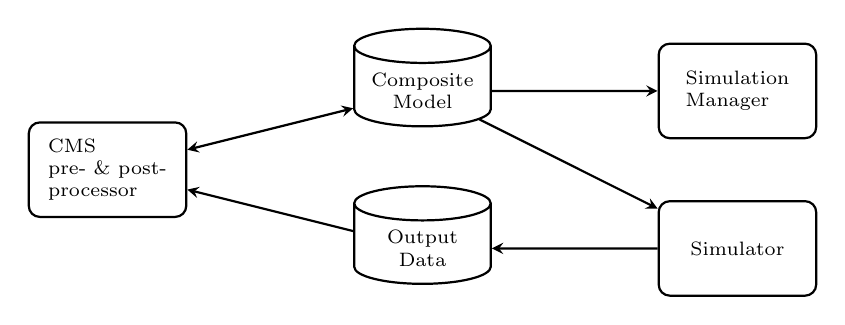
\begin{tikzpicture}[
		>=stealth,
		node distance=3cm,
		database/.style={
			cylinder,
			font=\scriptsize,
			text width=1.5cm,
			align=center,
			shape border rotate=90,
			aspect=0.25,
			draw,
			thick
		}
		]
		\node[database] (model) at (0,0) {Composite\\Model};
		\node[database] (data) at (0,-2cm) {Output\\Data};
		
		\node[rectangle,
			  draw,
			  thick,
			  rounded corners,
			  minimum width=2cm,
			  minimum height=1.2cm,
			  align=left,
			  font=\scriptsize] (manager) at (4cm,0) {Simulation\\Manager};
			  
  		\node[rectangle,
	  		  draw,
	          thick,
              rounded corners,
  		      minimum width=2cm,
  		      minimum height=1.2cm,
  		      align=left,
  		      font=\scriptsize] (simulator) at (4cm,-2cm) {Simulator};
  		      
  		\node[rectangle,
              draw,
  		      thick,
  		      rounded corners,
  		      minimum width=2cm,
  		      minimum height=1.2cm,
  		      align=left,
  		      font=\scriptsize] (cms) at (-4cm,-1cm) {CMS\\pre- \& post-\\processor};
  		
  		      
  		      
		
		\draw[<->,thick] (cms) -- (model);
		\draw[->,thick] (model) -- (manager);		
		\draw[->,thick] (model) -- (simulator);
		\draw[->,thick] (simulator) -- (data);
		\draw[->,thick] (data) -- (cms);
		%\draw[->,blue!50] (db1) -- ++(0,1) -- ($(db2)+(0,1)$) node[black,midway,above,font=\scriptsize]{Link: Name} node[black, midway,below,font=\scriptsize]{Owner: Name} -- (db2) ;
		\end{tikzpicture}
    %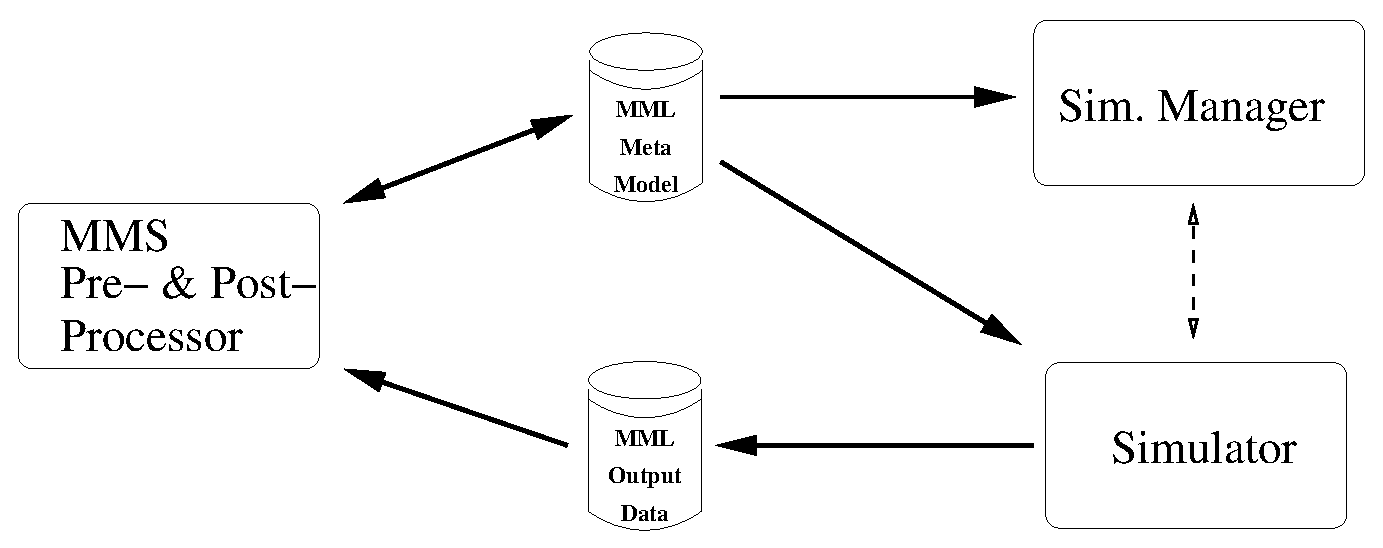
\epsfig{file=MetaModelSysDesign2.eps, width=10cm}
    \caption{The system design for the composite model simulation environment.} \label{fig:SystemDesign}
\end{center}\end{figure}%
%
\noindent In addition to the {\em simulation manager} a composite model {\em simulator} is included in the design that can start and monitor the
composite model simulation.
%It creates its own internal composite model
%structure for best simulation control and storage of composite model
%simulation results.
The simulation manager has been designed to act as a network server that allows several clients to connect and monitor the data flow between the interconnected external model simulators. 
The {\em simulator} can connect to this port. 
All data received by the simulation manager from the external model simulators is passed on to the simulator that stores results in the composite model output file.  
This client server architecture has some advantages over an integrated solution where the simulation manager is part of the simulator:
\begin{itemize}
%\item Improved performance of the simulation manager because all file
%	I/O is handled by the simulator.
\item The simulator and simulation manager can run on different machines, this is useful, for instance, if the simulation start up must	be performed on a machine other than the user's local machine.
\item Other processes can connect to the simulation manager's monitoring port. 
This allows, for instance, to visually monitor the co-simulation.
\end{itemize}

\noindent The simulation-manager manages start up of the different simulation tools (external model simulators) and communication between these tools, as defined by the simulation framework, see Figure~\ref{fig:MMSystem}. 
Each simulation tool implements the interface plug-in that handles the necessary communication with the simulation manager. 
The manager keeps an internal interconnection table for all connected external interfaces and forwards all received packages accordingly.

\begin{figure}[ht]\begin{center}
%    \setlength{\unitlength}{0.00087489in}
%
\begingroup\makeatletter\ifx\SetFigFont\undefined%
\gdef\SetFigFont#1#2#3#4#5{%
  \reset@font\fontsize{#1}{#2pt}%
  \fontfamily{#3}\fontseries{#4}\fontshape{#5}%
  \selectfont}%
\fi\endgroup%
{\renewcommand{\dashlinestretch}{30}
\begin{picture}(6048,5823)(0,-10)
\put(1344.377,3582.324){\arc{1245.924}{0.4048}{2.8429}}
\blacken\path(797.429,3329.777)(749.000,3399.000)(759.156,3315.130)(797.429,3329.777)
\put(3584.161,4223.729){\arc{562.723}{4.6869}{8.1023}}
\blacken\path(3660.873,4515.131)(3577.000,4505.000)(3655.773,4474.470)(3660.873,4515.131)
\put(4175.044,3639.532){\arc{979.217}{0.6661}{2.8971}}
\blacken\path(4519.208,3263.018)(4560.000,3337.000)(4489.192,3290.918)(4519.208,3263.018)
\put(2163.567,5181.406){\arc{749.004}{1.7359}{4.8745}}
\blacken\path(2141.124,5534.604)(2224.000,5551.000)(2143.158,5575.533)(2141.124,5534.604)
\put(3570.744,5190.695){\arc{757.493}{4.3990}{7.8375}}
\blacken\path(3655.674,4842.785)(3577.000,4812.000)(3660.905,4802.141)(3655.674,4842.785)
\put(453.521,3379.929){\arc{4279.820}{0.0201}{1.0142}}
\blacken\path(1641.400,1624.988)(1584.000,1563.000)(1663.818,1590.683)(1641.400,1624.988)
\put(-793.797,1402.000){\arc{8528.231}{5.8122}{6.4064}}
\blacken\path(3426.420,961.685)(3438.000,878.000)(3467.163,957.289)(3426.420,961.685)
\put(5622.020,3483.229){\arc{4836.890}{2.1368}{3.0811}}
\blacken\path(4245.323,1470.087)(4325.000,1442.000)(4267.914,1504.277)(4245.323,1470.087)
\put(2034.068,735.905){\arc{748.181}{1.7375}{4.8760}}
\blacken\path(2012.101,1088.720)(2095.000,1105.000)(2014.193,1129.647)(2012.101,1088.720)
\put(3352.880,740.063){\arc{759.917}{4.7232}{7.5128}}
\blacken\path(3544.918,436.064)(3480.000,382.000)(3562.723,399.153)(3544.918,436.064)
\path(1856,3951)(3700,3951)(3700,3337)
	(1856,3337)(1856,3951)
\path(4560,3951)(6036,3951)(6036,3091)
	(4560,3091)(4560,3951)
\put(4805,4135){\arc{120}{1.5708}{3.1416}}
\put(4805,4507){\arc{120}{3.1416}{4.7124}}
\put(5791,4507){\arc{120}{4.7124}{6.2832}}
\put(5791,4135){\arc{120}{0}{1.5708}}
\path(4745,4135)(4745,4507)
\path(4805,4567)(5791,4567)
\path(5851,4507)(5851,4135)
\path(5791,4075)(4805,4075)
\path(2102,5120)(3577,5120)(3577,4259)
	(2102,4259)(2102,5120)
\path(2224,5796)(3454,5796)(3454,4874)
	(2224,4874)(2224,5796)
\put(2346,5302){\arc{120}{1.5708}{3.1416}}
\put(2346,5674){\arc{120}{3.1416}{4.7124}}
\put(3332,5674){\arc{120}{4.7124}{6.2832}}
\put(3332,5302){\arc{120}{0}{1.5708}}
\path(2286,5302)(2286,5674)
\path(2346,5734)(3332,5734)
\path(3392,5674)(3392,5302)
\path(3332,5242)(2346,5242)
\path(12,4259)(1487,4259)(1487,3399)
	(12,3399)(12,4259)
\path(135,4935)(1365,4935)(1365,4013)
	(135,4013)(135,4935)
\put(257,4442){\arc{120}{1.5708}{3.1416}}
\put(257,4814){\arc{120}{3.1416}{4.7124}}
\put(1243,4814){\arc{120}{4.7124}{6.2832}}
\put(1243,4442){\arc{120}{0}{1.5708}}
\path(197,4442)(197,4814)
\path(257,4874)(1243,4874)
\path(1303,4814)(1303,4442)
\path(1243,4382)(257,4382)
\blacken\path(1506.466,2401.443)(1463.000,2329.000)(1535.443,2372.466)(1506.466,2401.443)
\path(1463,2329)(2471,3337)
\blacken\path(2427.534,3264.557)(2471.000,3337.000)(2398.557,3293.534)(2427.534,3264.557)
\blacken\path(1380.074,4593.404)(1303.000,4628.000)(1354.726,4561.204)(1380.074,4593.404)
\path(1303,4628)(2163,3951)
\blacken\path(2085.926,3985.596)(2163.000,3951.000)(2111.274,4017.796)(2085.926,3985.596)
\blacken\path(3310.510,4032.960)(3331.000,3951.000)(3351.490,4032.960)(3310.510,4032.960)
\path(3331,3951)(3331,5242)
\blacken\path(3351.490,5160.040)(3331.000,5242.000)(3310.510,5160.040)(3351.490,5160.040)
\blacken\path(3757.646,3705.760)(3700.000,3644.000)(3779.927,3671.366)(3757.646,3705.760)
\path(3700,3644)(4745,4321)
\blacken\path(4687.354,4259.240)(4745.000,4321.000)(4665.073,4293.634)(4687.354,4259.240)
\blacken\path(4491.453,2366.813)(4567.000,2329.000)(4518.135,2397.917)(4491.453,2366.813)
\path(4567,2329)(3392,3337)
\blacken\path(3467.547,3299.187)(3392.000,3337.000)(3440.865,3268.083)(3467.547,3299.187)
\blacken\path(2727.379,1645.172)(2747.000,1563.000)(2768.356,1644.739)(2727.379,1645.172)
\path(2747,1563)(2766,3358)
\blacken\path(2785.621,3275.828)(2766.000,3358.000)(2744.644,3276.261)(2785.621,3275.828)
\path(4345,1658)(5820,1658)(5820,797)
	(4345,797)(4345,1658)
\path(4468,2334)(5697,2334)(5697,1412)
	(4468,1412)(4468,2334)
\put(4589,1841){\arc{120}{1.5708}{3.1416}}
\put(4589,2213){\arc{120}{3.1416}{4.7124}}
\put(5575,2213){\arc{120}{4.7124}{6.2832}}
\put(5575,1841){\arc{120}{0}{1.5708}}
\path(4529,1841)(4529,2213)
\path(4589,2273)(5575,2273)
\path(5635,2213)(5635,1841)
\path(5575,1781)(4589,1781)
\path(4683,4648)(5913,4648)(5913,3726)
	(4683,3726)(4683,4648)
\path(128,1921)(1603,1921)(1603,1061)
	(128,1061)(128,1921)
\path(251,2597)(1480,2597)(1480,1675)
	(251,1675)(251,2597)
\put(372,2104){\arc{120}{1.5708}{3.1416}}
\put(372,2476){\arc{120}{3.1416}{4.7124}}
\put(1358,2476){\arc{120}{4.7124}{6.2832}}
\put(1358,2104){\arc{120}{0}{1.5708}}
\path(312,2104)(312,2476)
\path(372,2536)(1358,2536)
\path(1418,2476)(1418,2104)
\path(1358,2044)(372,2044)
\path(1982,872)(3457,872)(3457,12)
	(1982,12)(1982,872)
\path(2105,1549)(3334,1549)(3334,627)
	(2105,627)(2105,1549)
\put(2226,1056){\arc{120}{1.5708}{3.1416}}
\put(2226,1428){\arc{120}{3.1416}{4.7124}}
\put(3212,1428){\arc{120}{4.7124}{6.2832}}
\put(3212,1056){\arc{120}{0}{1.5708}}
\path(2166,1056)(2166,1428)
\path(2226,1488)(3212,1488)
\path(3272,1428)(3272,1056)
\path(3212,996)(2226,996)
\put(2471,3583){\makebox(0,0)[lb]{{\SetFigFont{8}{9.6}{\rmdefault}{\mddefault}{\updefault}Sim. Manager}}}
\put(4253,3337){\makebox(0,0)[lb]{{\SetFigFont{8}{9.6}{\rmdefault}{\mddefault}{\updefault}\emph{Start}}}}
\put(381,3214){\makebox(0,0)[lb]{{\SetFigFont{8}{9.6}{\rmdefault}{\mddefault}{\updefault}\emph{Start}}}}
\put(5114,3337){\makebox(0,0)[lb]{{\SetFigFont{8}{9.6}{\rmdefault}{\mddefault}{\updefault}Simulink}}}
\put(2655,4505){\makebox(0,0)[lb]{{\SetFigFont{8}{9.6}{\rmdefault}{\mddefault}{\updefault}Modelica}}}
\put(381,3644){\makebox(0,0)[lb]{{\SetFigFont{8}{9.6}{\rmdefault}{\mddefault}{\updefault}MSC.ADAMS}}}
\put(3823,4505){\makebox(0,0)[lb]{{\SetFigFont{8}{9.6}{\rmdefault}{\mddefault}{\updefault}\emph{Start}}}}
\put(1487,4505){\makebox(0,0)[lb]{{\SetFigFont{8}{9.6}{\rmdefault}{\mddefault}{\updefault} TLM data}}}
\put(2840,4075){\makebox(0,0)[lb]{{\SetFigFont{8}{9.6}{\rmdefault}{\mddefault}{\updefault} TLM data}}}
\put(3884,3706){\makebox(0,0)[lb]{{\SetFigFont{8}{9.6}{\rmdefault}{\mddefault}{\updefault} TLM data}}}
\put(1303,5242){\makebox(0,0)[lb]{{\SetFigFont{8}{9.6}{\rmdefault}{\mddefault}{\updefault}\parbox{10cm}{time step,\newline position,\newline velocity}}}}
\put(3700,4751){\makebox(0,0)[lb]{{\SetFigFont{8}{9.6}{\rmdefault}{\mddefault}{\updefault}Force, torque}}}
\put(4244,2692){\makebox(0,0)[lb]{{\SetFigFont{8}{9.6}{\rmdefault}{\mddefault}{\updefault} TLM data}}}
\put(1785,2571){\makebox(0,0)[lb]{{\SetFigFont{8}{9.6}{\rmdefault}{\mddefault}{\updefault} TLM data}}}
\put(3680,2128){\makebox(0,0)[lb]{{\SetFigFont{8}{9.6}{\rmdefault}{\mddefault}{\updefault}\emph{Start}}}}
\put(1987,2248){\makebox(0,0)[lb]{{\SetFigFont{8}{9.6}{\rmdefault}{\mddefault}{\updefault}\emph{Start}}}}
\put(3519,1603){\makebox(0,0)[lb]{{\SetFigFont{8}{9.6}{\rmdefault}{\mddefault}{\updefault}\emph{Start}}}}
\put(2753,2208){\makebox(0,0)[lb]{{\SetFigFont{8}{9.6}{\rmdefault}{\mddefault}{\updefault} TLM data}}}
\put(3761,515){\makebox(0,0)[lb]{{\SetFigFont{8}{9.6}{\rmdefault}{\mddefault}{\updefault}Force, torque}}}
\put(1100,354){\makebox(0,0)[lb]{{\SetFigFont{8}{9.6}{\rmdefault}{\mddefault}{\updefault}\parbox{5cm}{time step,\newline position,\newline velocity}}}}
\put(4898,1044){\makebox(0,0)[lb]{{\SetFigFont{8}{9.6}{\rmdefault}{\mddefault}{\updefault}Orpheus}}}
\put(2352,5481){\makebox(0,0)[lb]{{\SetFigFont{8}{9.6}{\rmdefault}{\mddefault}{\updefault}Interface plugin}}}
\put(237,4581){\makebox(0,0)[lb]{{\SetFigFont{8}{9.6}{\rmdefault}{\mddefault}{\updefault}Interface plugin}}}
\put(4602,1971){\makebox(0,0)[lb]{{\SetFigFont{8}{9.6}{\rmdefault}{\mddefault}{\updefault}Interface plugin}}}
\put(4782,4266){\makebox(0,0)[lb]{{\SetFigFont{8}{9.6}{\rmdefault}{\mddefault}{\updefault}Interface plugin}}}
\put(4782,3771){\makebox(0,0)[lb]{{\SetFigFont{8}{9.6}{\rmdefault}{\mddefault}{\updefault}Plugin wrapper}}}
\put(681,1306){\makebox(0,0)[lb]{{\SetFigFont{8}{9.6}{\rmdefault}{\mddefault}{\updefault}BEAST}}}
\put(2535,258){\makebox(0,0)[lb]{{\SetFigFont{8}{9.6}{\rmdefault}{\mddefault}{\updefault}BEAST}}}
\put(2217,1206){\makebox(0,0)[lb]{{\SetFigFont{8}{9.6}{\rmdefault}{\mddefault}{\updefault}Interface plugin}}}
\put(372,2241){\makebox(0,0)[lb]{{\SetFigFont{8}{9.6}{\rmdefault}{\mddefault}{\updefault}Interface plugin}}}
\put(417,1746){\makebox(0,0)[lb]{{\SetFigFont{8}{9.6}{\rmdefault}{\mddefault}{\updefault}Plugin wrapper}}}
\put(2217,711){\makebox(0,0)[lb]{{\SetFigFont{8}{9.6}{\rmdefault}{\mddefault}{\updefault}Plugin wrapper}}}
\put(4557,1476){\makebox(0,0)[lb]{{\SetFigFont{8}{9.6}{\rmdefault}{\mddefault}{\updefault}Plugin wrapper}}}
\put(2307,4941){\makebox(0,0)[lb]{{\SetFigFont{8}{9.6}{\rmdefault}{\mddefault}{\updefault}Plugin wrapper}}}
\put(237,4086){\makebox(0,0)[lb]{{\SetFigFont{8}{9.6}{\rmdefault}{\mddefault}{\updefault}Plugin wrapper}}}
\end{picture}
}

   {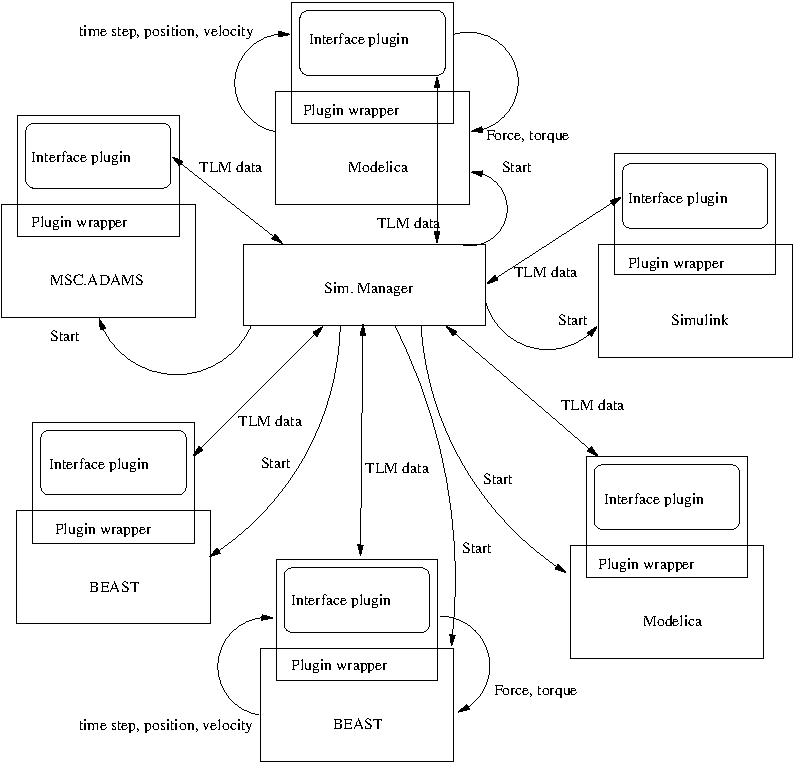
\includegraphics[width=9cm]{figs/TLM_system.pdf}}
    \caption{The simulation manager handles start up and communication between the tool specific simulators.}
    \label{fig:MMSystem}
\end{center}\end{figure}

Simulation results can be analysed in the post-processing applications, i.e., a two dimensional plotting program and a three dimensional visualisation tool, i.e., the composite model editor (CME). 
Data animation of system dynamics is possible to a limited extent based on the data that is exchanged in the external interfaces.

\section{Composite Model XML Files}
\label{meta}
The TLM default implementation contains a XML composite model reader, that can be used by the simulation manager to read the composite model from an XML file.

A composite model contains the following XML nodes:
\begin{description}
\item[Model] is the top composite model node that contains a list of {\tt SubModels} and {\tt Connections}.
\item[SubModels] is the node that contains the list of all {\tt SubModel} nodes.
\item[SubModel] is used for the external models. There is a {\tt SubModel} node for each external model that participates in the co-simulation. 
It defines a sub-model name used in the composite model and the start method and the simulation tool specific model files that needed to run the simulation. 
Each {\tt SubModel} node also contains a list of {\tt InterfacePoint} nodes.
\item[InterfacePoint] nodes are used to specify the TLM interfaces of each external model, that is, each {\tt SubModel}. 
It defines the name of a certain interface in the external model.
\item[Parameter] nodes specify {\tt SubModel} parameters which can be changed prior to simulation.
It defines the name of a certain interface in the external model.
\item[Connections] is the node that contains the list of all {\tt Connection} nodes.
\item[Connection] nodes define connections between two connected {\tt InterfacePoint}s, that is, a connection between two TLM interfaces. 
TLM parameters are specified for each connection.
\item[SimulationParams] node defines global composite model simulation parameters. 
Total simulation start time, end time, and network port  are defined in this node.
\end{description}


Here a sample composite model XML file for a Modelica with Beast co-simulation:
{\scriptsize
\begin{verbatim}
<?xml version="1.0" encoding="ISO-8859-1"?>

<!-- The root node is the composite model -->
<Model Name="Pendulum">

  <!-- List of connected sub-models -->
  <SubModels>	
    
    <!-- Each sub-model defines an external simulation model, 
         the following is an Modelica model that is started with
         the StartTLMModelica command and the model file shaft1.mo -->
    <SubModel Name="shaft1"
              StartCommand="StartTLMModelica" 
              ExactStep="0"
              ModelFile="shaft1.mo">
      
      <!-- TLM interface points for SubModel shaft1. 
	   For each interface one can define position and 
           orientation vectors. These are mainly useful for
           3D modeling. Orientation is defined as three angles
           aroung x, y, and z axis "x,y,z" in radians. Angle321
           defines rotation order 321 (z,y,x) of the three angles. 
	   Position and orientation is defined with respect to the 
	   external models inertial system. -->
      <InterfacePoint Name="tlm"
		      Position="0,-0.1,0"
		      Angle321="0,0,0"/>
    </SubModel>
    
    <!-- SubModel brg1. This is a BEAST model. Also for sub-models
	 one can define position and orientation vectors. These are
	 useful for translations between the different models.
	 Position and orientation is defined with respect to the composite
	 models global inertial system. -->
    <SubModel Name="brg1" 
              StartCommand="StartTLMBeast" 
              ExactStep="0"
              ModelFile="dgbb"
              Position="0,0,0"
              Angle321="1.5708,0,0">
      
      <!-- TLM interface points for SubModel brg1 -->
      <InterfacePoint Name="bIR`cs1"/>
      <InterfacePoint Name="bER`cs1"/>
    </SubModel>
    
    <!-- SubModel shaft2. This is another Modelica model. -->
    <SubModel Name="shaft2" 
              StartCommand="StartTLMModelica" 
              ExactStep="0"
              ModelFile="shaft2.mo">
      
      <!-- TLM interface points for SubModel C -->
      <InterfacePoint Name="tlm"/>
    </SubModel>    
  </SubModels>

  <!-- List of TLM connections -->
  <Connections>
    <!-- For each connections individual TLM parameters are defined.
	 Note, that the maximum step size must be smaller than the
	 shortest delay of all TLM connections for a single simulation
	 tool. This is taken care of by the tlmmanager. --> 
    <Connection From="shaft1.tlm" To="brg1.bER`cs1"
	 Delay="1e-3" Zf="1e4" Zfr="1e2" alpha="0.2"/>
    <!-- Each connections defines which interface of which models are 
         connected.
	 In these interfaces forces are exchanged, see TLM definition. -->
    <Connection From="shaft2.tlm" To="brg1.bIR`cs1" 
		Delay="1e-3" Zf="1e4" Zfr="1e2" alpha="0.2"/>
  </Connections>
  
  <!-- "Global" parameters for the co-simulation. 
       Typically the overall simulation time is defined here.
       This information is propageted to all simulation tools. 
       Note, some additional parameters for network port and 
       timeout can be defined here as well. But it is recommended 
       to not define this "system dependent settings" here.
       Use some system setup instead that can be given or read by 
       the tlmmanager.  -->
  <SimulationParams StartTime="0.0" 
                    StopTime="1.0"/>
  
</Model>
\end{verbatim}
}
